\likechapter{Введение}

Шагающие роботы - это класс роботов, имитирующих движения людей и животных. Миллионы лет эволюции показывают, что передвижение при помощи ног это наиболее эффективный способ быстро приспосабливаться к плохим, неровным поверхностям. Сегодня от робототехнической шагающей системы требуется приспосабливаться к тем условиям, в которых она раньше не была. Рассмотрим существующих роботов, которые сегодня есть на рынке, и то, каким образом их разработчики решают эту задачу.

\textbf{Рынок шагающих роботов}

Классифицировать шагающие машины можно не только по количеству ног. Некоторые роботы комплектуются также и колесами, для увеличения скорости передвижения по ровным поверхностям. Для простоты, разделим рассматриваемых роботов на двуногих и четырехногих. 

На текущий момент можно найти огромное количество шагающих роботов. Гексаподы, робо-пауки и т.д. Но среди сотен моделей можно выделить таких, ходьба которых максимально приближена к животной.

Среди современных четырехногих роботов можно выделить:
\begin{itemize}
    \item роботы Spot и Spot-Mini от компании Boston Dynamics \cite{BostonDynamics2020} (рисунок~\ref{fig:intro1});
    \item робот Mini-Cheetah от студентов MIT \cite{Mit2020};
    \item Робот ANYmal от студентов Цюрихского университета \cite{ZurichETH2020} (рисунок~\ref{fig:intro2});
    \item робот HyQReal от IIT \cite{Iit2020} (Итальянского технологического института);
    \item роботы LaikaGo и AlienGo от компании Unitree Robotics \cite{Unitree2020}.
\end{itemize}

\begin{figure}[h!]
    \centering
    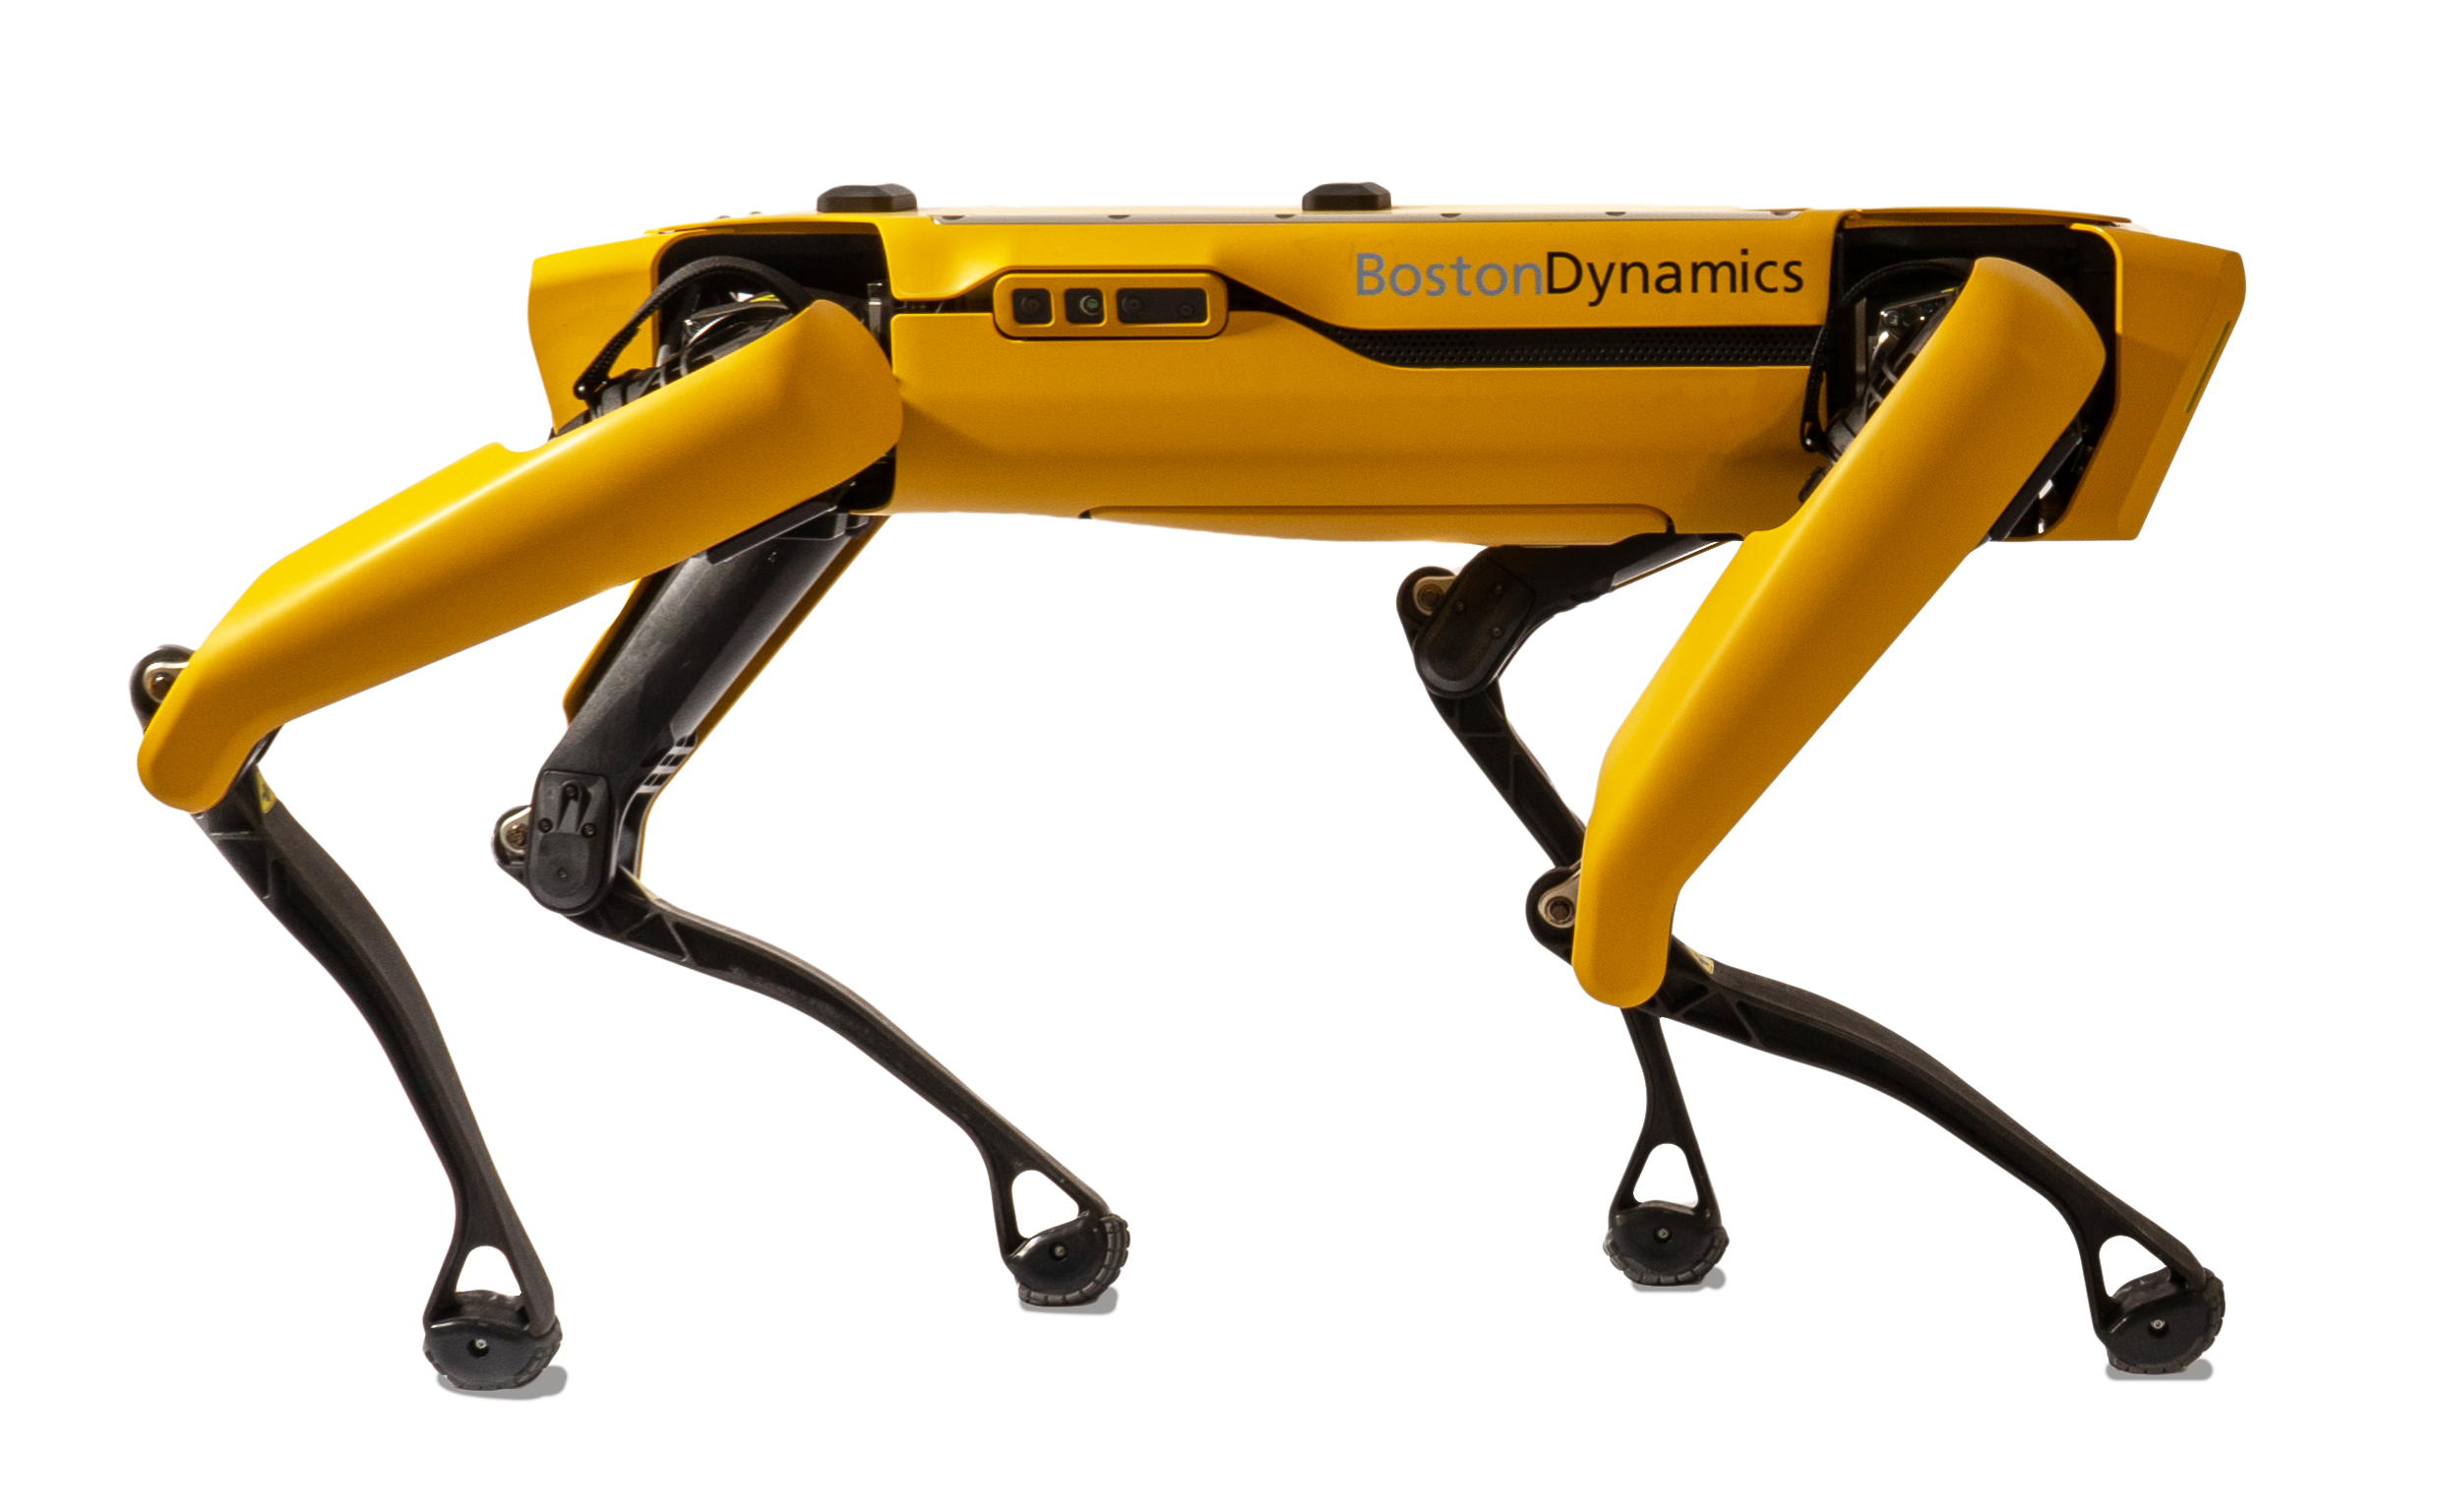
\includegraphics[width=0.6\textwidth]{chapter_intro/figure1.png}
    \caption{Робот \textit{Spot-mini} компании \textit{Boston Dynamics}}
    \label{fig:intro1}
\end{figure}

\begin{figure}[h!]
    \centering
    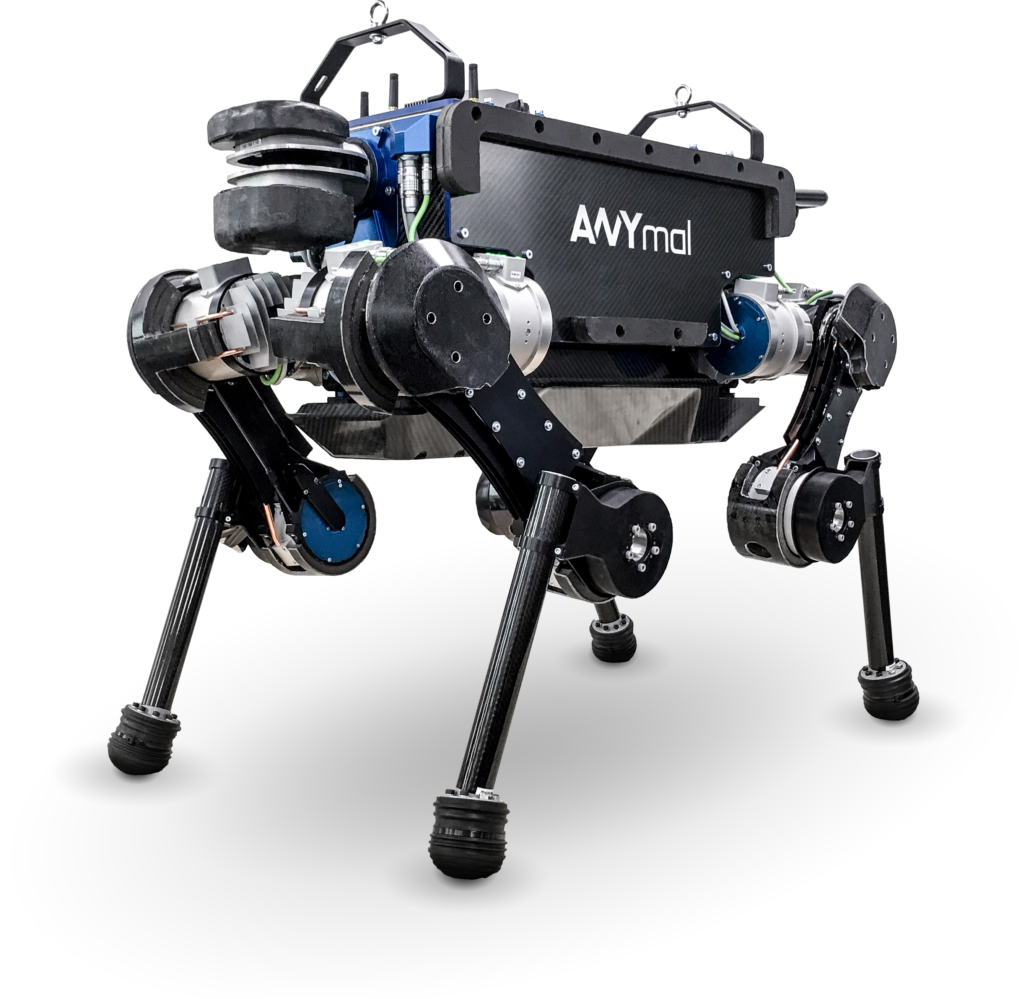
\includegraphics[width=0.6\textwidth]{chapter_intro/figure2.png}
    \caption{Робот \textit{ANYmal} университета \textit{ ETH Zurich}}
    \label{fig:intro2}
\end{figure}

Среди двуногих можно выделить такие проекты, как:

\begin{itemize}
    \item робот Digit от компаний Agility Robotics и Ford \cite{Agility2020_2} (рисунок~\ref{fig:intro3});
    \item робот Cassie от компании Agility Robotics \cite{Agility2020_2};
    \item робот Atlas от компании Boston Dynamics \cite{BostonDynamics2020}.
\end{itemize}

\begin{figure}[h]
    \centering
    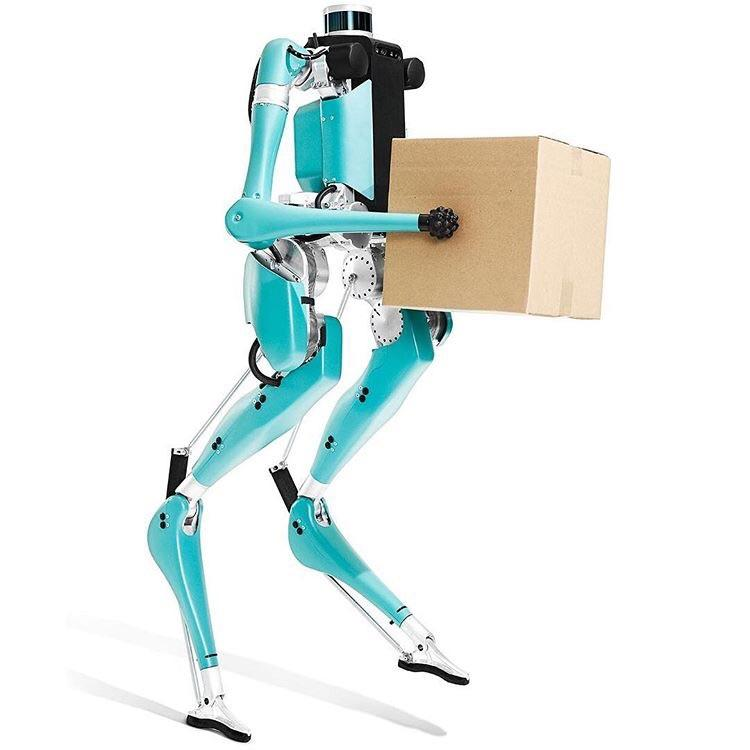
\includegraphics[width=0.6\textwidth]{chapter_intro/figure3.jpg}
    \caption{Робот \textit{Digit} компании \textit{ Agility Robotics}}
    \label{fig:intro3}
\end{figure}

\begin{figure}[h]
    \centering
    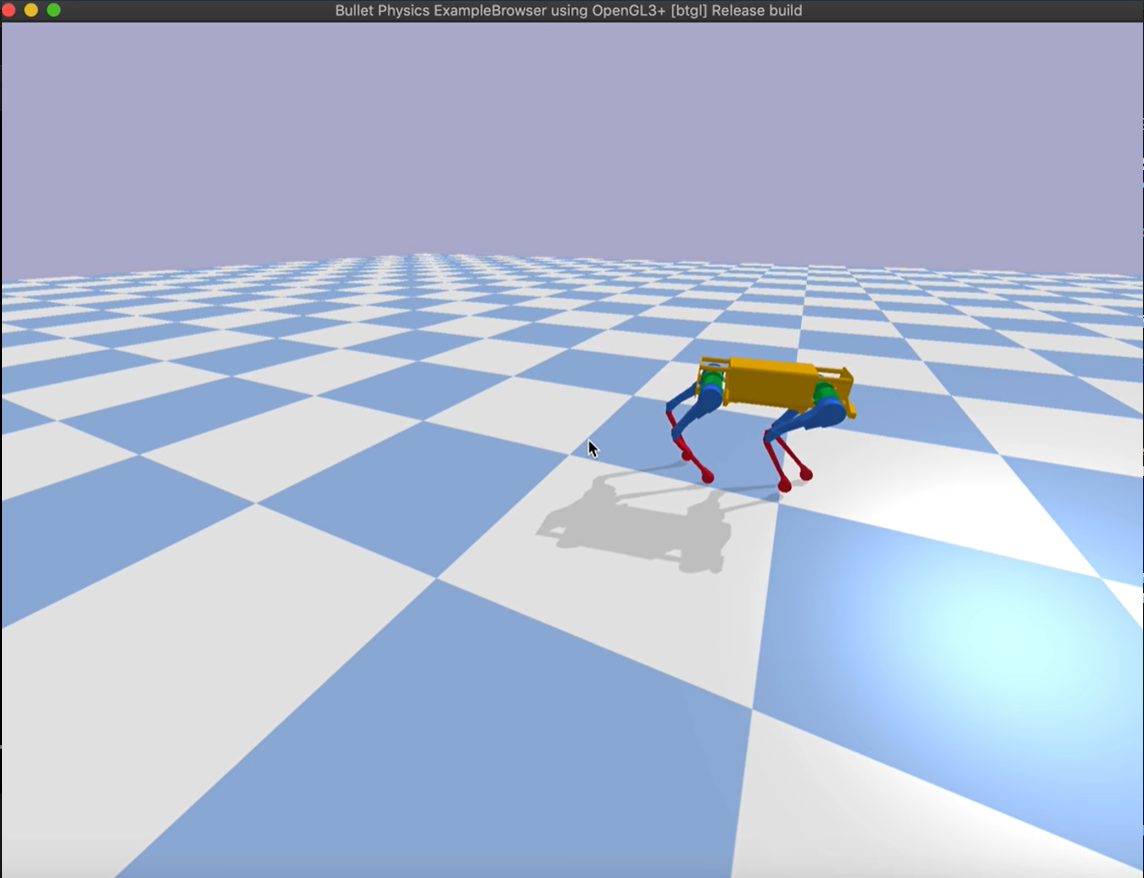
\includegraphics[width=0.95\textwidth]{chapter_intro/figure5.png}
    \caption{Обучение ходьбе в симуляции робота \textit{LaikaGo} компании \textit{ Unitree Robotics} }
    \label{fig:intro4}
\end{figure}

Всех выше перечисленных роботов объединяет одна схожая особенность -- они обучены ходьбе при помощи новых, набирающих популярность, методов глубокого обучения. Алгоритм их ходьбы не описан статическими константами в коде, он создан при помощи обучения моделей искусственных нейронных сетей. Благодаря этому все они показывают высокую степень мобильности и адаптивности к окружающей среде. Далее, для некоторых из роботов, приведены используемые разработчиками методы обучения. Движения таких роботов при перемещении визуально похожи на движения животных со схожим механическим строением тела. 
Стоит отметить, что модели, обученные таким образом показывают более высокую эффективность при перемещении \cite{Hwangbo2019} и меньшее потребление энергии, чем модели ходьбы, описанные человеком вручную.

\begin{figure}[h!]
    \centering
    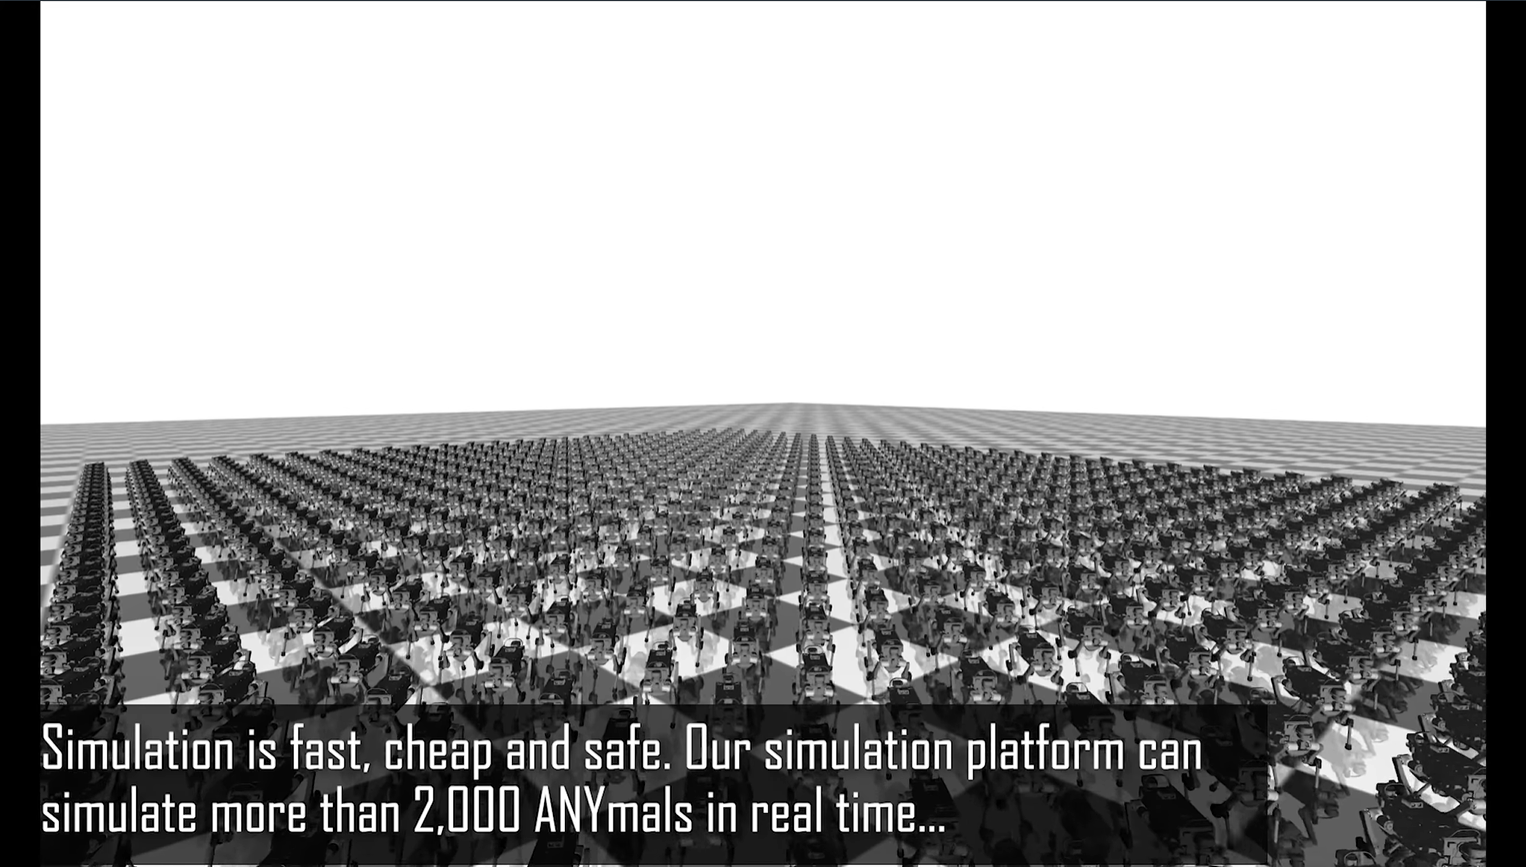
\includegraphics[width=0.95\textwidth]{chapter_intro/figure6.png}
    \caption{Множество моделей робота \textit{ANYmal} обучаются одновременно }
    \label{fig:intro5}
\end{figure}

Для обучения четырехногого робота LaikaGo используется помещенная в симуляцию физическая модель робота \cite{LaikaGo2019} (рисунок \ref{fig:intro4}). Робот ANYmal точно так же был <<натренирован>> при помощи многократных запусков его физической модели в симуляции. Чтобы ускорить процесс, разработчики поместили в симуляцию сразу множество физических моделей робота, которые тренировались одновременно \cite{RoboSysLab2019}. Такой способ позволил быстро, дешево и безопасно обучать робота ходьбе (демонстрация метода на рисунке~\ref{fig:intro5}). 

Такую же схему обучения используют для двуногого робота Cassie \cite{AgilityRobo2018}. Кроме того, разработчики из Agility Robotics используют машинное обучение еще и для планирования траектории, а также для правильного позиционирования стоп робота на неровной местности \cite{Agility2020}.

Для большинства приведенных выше четырехногих роботов можно также выявить одну общую особенность -- у них схожие кинематические схемы, у конечностей по три степени свободы. Отсутствие избыточных степеней свободы упрощает проектирование конечностей и разработку математических моделей их движения. Этот факт повлиял на конструкцию ног робота, которая была разработана в рамках данного проекта.

\section*{Актуальность работы}

Задача разработки шагающих роботов становится все более актуальной с каждым годом. Всё в большей степени людей стараются заменять шагающими роботами для работ, в которых требуется мобильность и подвижность человеческих ног, и при этом невозможно присутствие самого человека. Например, приведенные выше роботы создаются для инспекции строек и помещений, исследования местности вдали от дорог и цивилизации, помощи в устранении последствий катастроф, пребывания в опасной для человека среде (под воздействием вредных газов, излучения). Также недавно появился опыт применения таких роботов для уменьшения количества контактов между людьми во время эпидемии респираторного заболевания \cite{Bbc2020}. Открытость методик, исходных кодов и готовых моделей в открытом доступе приведет к массовой разработке шагающих роботов не только крупными предприятиями, но и частными разработчиками. 

%\fixme ОБЗОР РЫНКА И АНАЛИЗ ЛИТЕРАТУРЫ
